\documentclass[11pt]{article}

\usepackage[margin=2.5cm]{geometry}
\usepackage{authblk}
\usepackage{booktabs}
\usepackage{microtype}
\usepackage{siunitx}
\usepackage{hyperref}
\usepackage{natbib}
\usepackage{xcolor}
\usepackage{pgfplots}
\pgfplotsset{compat=1.18}

\hypersetup{colorlinks=true,linkcolor=black,citecolor=black,urlcolor=blue}
\newcommand{\BenchmarkScenarioCount}{31}
\newcommand{\BenchmarkExactScenarioCount}{31}
\newcommand{\MedianSpeedup}{45.2}
\newcommand{\MinimumSpeedup}{31.3}
\newcommand{\MaximumSpeedup}{50.5}
\newcommand{\MedianTallyTime}{0.42}
\newcommand{\MedianHTSeqTime}{18.64}
\newcommand{\MedianTallyRSS}{28.5}
\newcommand{\MedianHTSeqRSS}{72.1}
\newcommand{\MedianMemoryRatio}{2.55}
\newcommand{\BenchmarkDataset}{Pasilla Drosophila chromosome 4}
\newcommand{\BenchmarkRunId}{36193504716}
\newcommand{\BenchmarkCommit}{ad54b53a}

\newcommand{\ScalingRepeats}{5}
\newcommand{\ScalingMaxRecords}{10000000}
\newcommand{\ScalingTallyTenMTime}{10.02}
\newcommand{\ScalingHTSeqTenMTime}{221.74}
\newcommand{\ScalingTenMSpeedup}{22.1}
\newcommand{\ScalingTallySlope}{0.964}
\newcommand{\ScalingHTSeqSlope}{20.911}
\newcommand{\ScalingTallyIntercept}{0.396}
\newcommand{\ScalingHTSeqIntercept}{7.117}
\newcommand{\ScalingTallyRSquared}{0.9998}
\newcommand{\ScalingHTSeqRSquared}{0.9931}


\title{TallySeq: a high-performance, HTSeq-compatible read counting tool in Rust}
\author[1]{Cedric Hermans}
\affil[1]{BIT\textsuperscript{2}lab, Howest University of Applied Sciences, Bruges, Belgium}
\date{}

\begin{document}
\maketitle

\begin{abstract}
Read summarization against genomic annotations remains a routine step in sequencing workflows. \texttt{htseq-count} is widely used because its treatment of strandedness, ambiguous overlaps, multimapping reads, paired-end fragments, and annotation attributes is well established, but its runtime can become substantial when many alignments are processed. We present TallySeq, a Rust implementation designed to reproduce HTSeq 2.1.2 counting semantics while reducing runtime and memory use. TallySeq supports single- and paired-end SAM/BAM input, CRAM on Linux and macOS, the three HTSeq overlap modes, strandedness modes, nonunique-read handling, multi-file processing, annotation metadata, annotated SAM/BAM output, and tabular, Matrix Market, H5AD, and Loom count output. Correctness is assessed by differential tests against HTSeq 2.1.2, targeted interval and CIGAR edge cases, upstream HTSeq fixtures, and real-data scenarios. In a repeated real-data benchmark using two Drosophila Pasilla chromosome 4 datasets and the matching Ensembl annotation, all \BenchmarkExactScenarioCount{} dataset--scenario comparisons across \BenchmarkScenarioCount{} scenarios produced exactly identical count tables. Each tool was run \BenchmarkRepeats{} times per comparison with single-thread settings. Across dataset--scenario medians, TallySeq required \SI{\MedianTallyTime}{\second} compared with \SI{\MedianHTSeqTime}{\second} for HTSeq, a median \MedianSpeedup{}-fold speed ratio (range \MinimumSpeedup{}--\MaximumSpeedup{}). Median peak resident memory was \MedianTallyRSS{}~MiB and \MedianHTSeqRSS{}~MiB, respectively. In controlled read-count scaling to 10 million alignments, median runtime was \SI{\ScalingTallyTenMTime}{\second} for TallySeq and \SI{\ScalingHTSeqTenMTime}{\second} for HTSeq. Linear fits gave slopes of \ScalingTallySlope{} and \ScalingHTSeqSlope{} seconds per million alignments, respectively.
\end{abstract}

\section{Introduction}

Assigning aligned sequencing reads or fragments to genomic features is conceptually simple but becomes complicated at exon boundaries, overlapping genes, splice junctions, multimapping alignments, paired-end fragments, and strand-specific protocols. HTSeq introduced a general Python framework for high-throughput sequencing data and the \texttt{htseq-count} command for gene-level read summarization \citep{Anders2015}. HTSeq 2.0 subsequently expanded \texttt{htseq-count} with multi-file processing, additional annotation metadata, sparse output representations, and modernized I/O and deployment \citep{Putri2022}.

Other high-performance read summarizers exist, including featureCounts \citep{Liao2014}. TallySeq addresses a narrower compatibility goal: preserve the established command-line behavior and counting semantics of \texttt{htseq-count} while reducing the computational cost of workflows that already depend on those semantics. This makes performance improvements useful without requiring users to reinterpret differences caused by a different counting model.

TallySeq is implemented in Rust and exposes both a \texttt{tallyseq} executable and an \texttt{htseq-count} compatibility executable in release archives. The implementation has been developed together with a differential test suite that compares counts and compatibility outputs against HTSeq 2.1.2.

\section{Implementation}

\subsection{Counting model}

TallySeq reproduces the three HTSeq overlap modes: \texttt{union}, \texttt{intersection-strict}, and \texttt{intersection-nonempty}. It supports \texttt{yes}, \texttt{no}, and \texttt{reverse} strandedness; single- and paired-end alignments; name- and coordinate-sorted paired-end input; MAPQ filtering; handling of secondary and supplementary alignments; and the HTSeq \texttt{none}, \texttt{all}, \texttt{fraction}, and \texttt{random} policies for nonunique feature assignments.

Alignment blocks are derived from reference-consuming CIGAR operations. Insertions and clipping do not advance reference coordinates, while deletions and skipped regions advance the reference without being counted as aligned blocks. Paired-end reads are summarized as fragments, consistent with the behavior described for \texttt{htseq-count} \citep{Anders2015}.

\subsection{Annotation indexing}

GTF/GFF annotation is parsed once per invocation. Feature names are interned and represented internally by integer identifiers, while chromosome-specific interval trees are immutable and shared between input files. A multi-file invocation therefore reuses the same annotation index instead of reparsing the GTF for every sample. This design mirrors the load-once motivation of HTSeq 2.0 multi-file counting \citep{Putri2022}, while allowing concurrent processing of alignment files.

The interval query implementation performs a single pruned range traversal using subtree maximum-end coordinates. Each interval is stored once in the tree, so overlap queries can return matching features without a separate sort-and-deduplicate pass.

\subsection{I/O and output compatibility}

Local SAM and BAM files use a lightweight Rust reader on the normal counting path. On Linux and macOS, HTSlib is used as a compatibility bridge for CRAM, standard input, and content-based format conversion. The Windows build uses the Rust SAM/BAM path and does not currently support CRAM.

TallySeq supports multiple alignment files, compressed GTF/GFF input, repeated feature types and ID attributes, annotation metadata columns, feature queries, and HTSeq-style annotated SAM/BAM output via the \texttt{XF} tag. Count output can be written as delimited text, Matrix Market, H5AD, or Loom. Release packages contain both the native \texttt{tallyseq} command and a compatibility copy named \texttt{htseq-count}.

\section{Correctness validation}

Correctness testing is differential by design. Generated SAM/GTF cases are executed with both TallySeq and HTSeq and the complete count tables are compared. The current suite contains 292 generated single- and paired-end cases, including fuzz-generated combinations of CIGAR operations, flags, MAPQ values, NH tags, overlap modes, and strandedness options. Fourteen additional adversarial interval cases exercise one-base features, adjacent and overlapping exons, deletions, splice gaps, clipping, and strand boundaries. Six scenarios derived from the upstream HTSeq reference fixtures are also compared.

A separate compatibility suite covers multi-file counting, headers and append behavior, compressed annotations, GFF3 attributes, duplicate annotation attributes, feature queries, multiple ID attributes, CRAM, standard input, SAM/BAM annotation output, H5AD, Loom, and Matrix Market output. Real-data benchmark scenarios are accepted only when every feature row and every HTSeq special row has exactly the same numeric count. No numerical tolerance is used for the count comparison.

\section{Benchmark design}

\subsection{Real-data compatibility and performance matrix}

The benchmark uses the Pasilla RNA-seq training data deposited in Zenodo record 61771 \citep{Gruning2016}. Two paired-end chromosome 4 datasets, \texttt{GSM461177} and \texttt{GSM461178}, are downloaded together with \texttt{Drosophila\_melanogaster.BDGP5.78.gtf}, and all source files are checksum-verified. For each dataset, a single-end BAM is reproducibly derived from mate 1 while retaining alignment coordinates, CIGAR strings, MAPQ values, sequence, strand, and auxiliary tags. A query-name-sorted paired BAM is also generated for the name-order scenario.

The full matrix contains \BenchmarkScenarioCount{} scenarios per dataset. The core matrix combines single- and paired-end input with all three overlap modes and all three strandedness modes. Targeted scenarios cover \texttt{--nonunique all}, \texttt{--nonunique fraction}, MAPQ threshold changes, scoring of secondary and supplementary alignments, repeated feature types, repeated ID attributes, and paired-end name sorting. \texttt{--nonunique random} is excluded from exact differential benchmarking because TallySeq and HTSeq use independent random-number generators. Annotated alignment output is tested in the compatibility suite rather than timed in this count-performance matrix because writing SAM/BAM adds a separate output-I/O workload.

Every dataset--scenario combination must pass exact feature-key and numeric count equality before timings are accepted. Row order is normalized and no numerical tolerance is used. Each accepted combination is then measured \BenchmarkRepeats{} times for each tool. TallySeq is run with \texttt{--threads \BenchmarkTallyThreads}; both tools use \texttt{-n \BenchmarkNProcesses}. Tool execution order is alternated by repeat to reduce systematic page-cache bias. Wall-clock time and maximum resident set size are recorded with GNU \texttt{/usr/bin/time}.

Measurements were collected with TallySeq 0.1.0 and HTSeq 2.1.2 on an Intel Core i7-9750H CPU (12 logical CPUs) with 15.5~GiB RAM under Linux 6.18.33.2 in WSL2. Benchmark data were stored on an ext4 filesystem. The Rust toolchain was rustc 1.98.1, and the benchmarked repository state was commit \texttt{8d0dd196}.

\subsection{Controlled read-count scaling}

A second benchmark isolates the effect of alignment count. It starts from the real \texttt{GSM461177} mate-1 single-end records and deterministically cycles those records until inputs contain exactly 100,000, 1,000,000, 5,000,000, and 10,000,000 alignments. The scaling step does not synthesize or modify coordinates, CIGAR strings, MAPQ values, tags, strands, or sequences, so the alignment distribution is held fixed while the number of records changes.

Both tools use union, unstranded exon counting by \texttt{gene\_id} at MAPQ $\geq 10$, with secondary and supplementary alignments ignored and nonunique assignment set to \texttt{none}. Each target is measured \ScalingRepeats{} times per tool with the same single-thread settings and alternating execution order as the real-data matrix. Exact count equality is required for every target and repeat. Linear least-squares fits are calculated from median wall time against alignment count in millions.

\section{Results}

\subsection{Count parity}

All \BenchmarkDatasetScenarioCount{} dataset--scenario comparisons produced exactly identical count tables between TallySeq and HTSeq 2.1.2. This covers the three overlap modes, three strandedness settings, single- and paired-end processing, coordinate- and name-sorted paired input, multimapper policies, MAPQ changes, secondary and supplementary alignments, multiple feature types, and compound feature identifiers. The scaling benchmark also produced exact equality at every record count and repeat.

\subsection{Runtime and memory}

Across the \BenchmarkDatasetScenarioCount{} dataset--scenario comparisons, the median of the per-comparison median runtimes was \SI{\MedianTallyTime}{\second} for TallySeq and \SI{\MedianHTSeqTime}{\second} for HTSeq. The median pairwise speed ratio was \MedianSpeedup{}-fold, with a range of \MinimumSpeedup{}--\MaximumSpeedup{}-fold. Median peak resident memory was \MedianTallyRSS{}~MiB for TallySeq and \MedianHTSeqRSS{}~MiB for HTSeq, corresponding to a median HTSeq/TallySeq memory ratio of \MedianMemoryRatio{}.

\begin{table}[ht]
\centering
\caption{Summary of the repeated real-data benchmark. Values are medians across dataset--scenario medians; each dataset--scenario median is based on five runs per tool. The single-end, paired-end, core, and targeted rows are overlapping subsets of the full matrix.}
\label{tab:benchmark}
\begin{tabular}{lrrrrrr}
\toprule
Subset & Comparisons & \multicolumn{2}{c}{Time (s)} & Speed ratio & \multicolumn{2}{c}{Peak RSS (MiB)} \\
\cmidrule(lr){3-4}\cmidrule(lr){6-7}
 & & TallySeq & HTSeq & $\times$ & TallySeq & HTSeq \\
\midrule
All & 62 & 0.58 & 14.59 & 26.1 & 28.1 & 73.8 \\
Single-end & 30 & 0.50 & 13.68 & 27.5 & 25.8 & 67.6 \\
Paired-end & 32 & 0.60 & 14.86 & 25.2 & 29.6 & 76.4 \\
Core matrix & 36 & 0.58 & 14.62 & 26.4 & 27.0 & 70.7 \\
Targeted options & 26 & 0.58 & 14.53 & 25.6 & 28.1 & 74.1 \\
\bottomrule
\end{tabular}
\end{table}

The smallest pairwise speed ratio, 18.7-fold, occurred for paired-end counting with the compound \texttt{gene\_id:transcript\_id} identifier in \texttt{GSM461178}. The largest, 29.1-fold, occurred for single-end, intersection-strict, stranded counting in \texttt{GSM461177}. Compound identifiers increased memory use in both tools because they expand the number of distinct output features.

\subsection{Read-count scaling}

Runtime increased approximately linearly with alignment count for both tools (Table~\ref{tab:scaling}). At 10 million alignments, TallySeq completed in a median \SI{\ScalingTallyTenMTime}{\second}, while HTSeq required \SI{\ScalingHTSeqTenMTime}{\second}, a \ScalingTenMSpeedup{}-fold ratio.

\begin{table}[ht]
\centering
\caption{Controlled read-count scaling using cyclic repetition of real \texttt{GSM461177} single-end alignments. Each value is the median of five runs, and every run passed exact count equality.}
\label{tab:scaling}
\begin{tabular}{rrrrrrr}
\toprule
Records & BAM (MiB) & \multicolumn{2}{c}{Time (s)} & Speed ratio & \multicolumn{2}{c}{Peak RSS (MiB)} \\
\cmidrule(lr){3-4}\cmidrule(lr){6-7}
 & & TallySeq & HTSeq & $\times$ & TallySeq & HTSeq \\
\midrule
100,000 & 2.35 & 0.53 & 14.65 & 27.6 & 25.8 & 67.6 \\
1,000,000 & 23.82 & 1.29 & 28.25 & 21.9 & 25.8 & 67.6 \\
5,000,000 & 119.06 & 5.27 & 100.50 & 19.1 & 25.9 & 67.7 \\
10,000,000 & 238.09 & 10.02 & 221.74 & 22.1 & 25.8 & 67.5 \\
\bottomrule
\end{tabular}
\end{table}

Writing runtime as $t = a + bN$, where $N$ is the number of alignments in millions, the TallySeq fit gave $a=\ScalingTallyIntercept{}$~s and $b=\ScalingTallySlope{}$~s per million alignments ($R^2=\ScalingTallyRSquared$). The HTSeq fit gave $a=\ScalingHTSeqIntercept{}$~s and $b=\ScalingHTSeqSlope{}$~s per million alignments ($R^2=\ScalingHTSeqRSquared$). The fitted per-million-record slope was therefore about 21.7 times larger for HTSeq. Peak resident memory remained nearly constant across the four record counts for both tools.

\begin{figure}[ht]
\centering
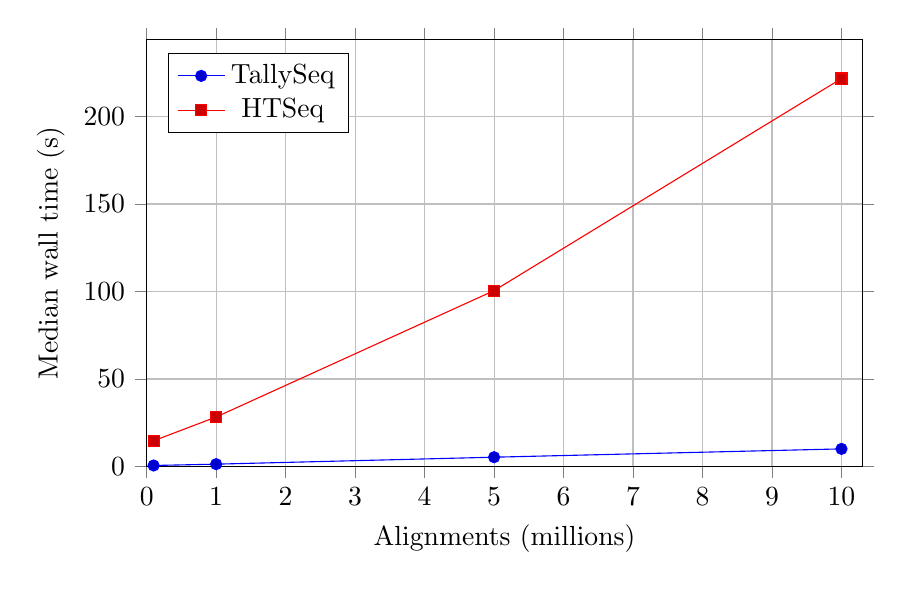
\begin{tikzpicture}
\begin{axis}[
    width=0.88\linewidth,
    height=7.0cm,
    xlabel={Alignments (millions)},
    ylabel={Median wall time (s)},
    xmin=0,
    xmax=10.3,
    ymin=0,
    grid=major,
    legend pos=north west,
    tick align=outside,
]
\addplot+[mark=*] coordinates {
    (0.1,0.53)
    (1,1.29)
    (5,5.27)
    (10,10.02)
};
\addlegendentry{TallySeq}
\addplot+[mark=square*] coordinates {
    (0.1,14.65)
    (1,28.25)
    (5,100.50)
    (10,221.74)
};
\addlegendentry{HTSeq}
\end{axis}
\end{tikzpicture}
\caption{Controlled read-count scaling. Each point is the median of five runs after exact count equality was confirmed. The input alignment distribution is held constant by deterministic repetition of real Pasilla records.}
\label{fig:scaling}
\end{figure}

\section{Discussion}

The differential tests and real-data benchmarks support the main compatibility goal: TallySeq reproduces HTSeq 2.1.2 count output across the tested overlap modes, strandedness modes, paired-end orderings, multimapper policies, filtering options, and annotation configurations. Exact equality is checked before a benchmark timing is accepted, so the performance comparison is tied directly to equivalent count output.

The runtime difference is visible in both the small real-data matrix and the controlled scaling experiment. The scaling fit is especially informative because the alignment distribution and annotation are held constant while only the number of records changes. TallySeq's fitted slope of \ScalingTallySlope{} seconds per million alignments is substantially lower than HTSeq's \ScalingHTSeqSlope{} seconds per million. The fitted intercepts also differ, although they should be interpreted only as regression parameters rather than direct measurements of annotation parsing or startup cost.

TallySeq's counting path uses integer feature identifiers, immutable chromosome-specific interval trees, pruned range queries, reusable alignment buffers, and limited allocation of temporary strings. Multi-file invocations share one parsed annotation index and can process alignment inputs concurrently. These design choices reduce work in the hot path while retaining HTSeq-compatible assignment rules.

The benchmark results are most useful for workflows that already rely on \texttt{htseq-count} semantics. TallySeq is not intended to define a new quantification model. Other read summarizers can make different assignment choices, so runtime comparisons without matching semantics would answer a different question.

\section{Limitations}

TallySeq targets the \texttt{htseq-count} command rather than the complete HTSeq Python API. CRAM input is unavailable in the native Windows package because its CRAM compatibility path depends on HTSlib. The \texttt{--nonunique random} mode is implemented, but individual ambiguous-read assignments are not expected to match exactly because TallySeq and HTSeq use independent random-number generators.

Performance measurements were collected on one x86\_64 workstation under WSL2 with one TallySeq decoding thread and one alignment-processing process for both tools. Absolute runtimes will vary with processor, storage, operating system, and file compression. The benchmark does not measure multi-file parallel throughput, CRAM performance, or annotated SAM/BAM output throughput.

The scaling inputs deliberately repeat real alignment records to hold the alignment distribution constant. This isolates read-count scaling, but it does not reproduce increasing genomic diversity, annotation complexity, or the compression characteristics of an independently sequenced 10-million-read dataset. The benchmark therefore supports conclusions about scaling with record count under a controlled workload, not every property of large sequencing datasets.

\section{Availability}

TallySeq source code, benchmark scripts, differential tests, and release packaging are available at \url{https://github.com/CedricHermansBIT/TallySeq}. The repository includes a reproducible real-data benchmark that downloads and checksum-verifies its input data, rejects any benchmark run with unequal counts, and reports wall-clock time and peak resident memory.

\section{Author contributions}

Cedric Hermans: conceptualization, software, methodology, validation, benchmarking, and writing of the initial manuscript draft.

\section{Competing interests}

The author declares no competing interests.

\bibliographystyle{plainnat}
\bibliography{references}

\end{document}
